
\label{sec:eva}
Our evaluation focuses on four research questions:
{\bf RQ1}: Can \Tool identify view-aware optimization opportunities from latest versions
    of popular web applications?
{\bf RQ2}: How much performance benefits can view-aware optimization provide?
{\bf RQ3}: Is the performance-functionality trade-off space exposed by \Tool worthwhile for developers to explore?
{\bf RQ4}: Does \Tool estimator estimate the per-tag data-processing cost accurately?
\begin{table}[t]											
\centering											
\caption{Opportunities detected by \Tool in 12 apps}												
\label{tab:oppo}										\centering
\resizebox{0.6\columnwidth}{!}{%
\begin{tabular}{@{}lrrrrrrrrrrrrr@{}}
\toprule
App	&	Ds	&	Lo	&	Gi	&	Re	&	Sp	&	Ro	&	Fu	&	Tr	&	Da	&	On	&	FF	&	OS	&	SUM	\\	\midrule
pagi.	&	1	&	6	&	1	&	10	&	2	&	20	&	5	&	9	&	1	&	6	&	3	&	3	&	69	\\	\midrule
approx.	&	1	&	1	&	0	&	7	&	0	&	5	&	1	&	3	&	0	&	23	&	0	&	0	&	43	\\	\midrule
removal	&	1	&	2	&	0	&	7	&	0	&	4	&	1	&	2	&	2	&	2	&	0	&	0	&	22	\\	\midrule
asynch	&	1	&	2	&	0	&	2	&	0	&	2	&	1	&	2	&	2	&	2	&	0	&	0	&	15	\\	\midrule
SUM	&	4	&	11	&	1	&	26	&	2	&	31	&	8	&	16	&	5	&	33	&	3	&	3	&	149	\\	
 \bottomrule
\end{tabular}

}	
\end{table}

\begin{table}[h]
\centering
\caption{Speed up of 15 view changes}
\label{tab:speedup}
\resizebox{\columnwidth}{!}{%
\begin{tabular}{@{}l|rrrrrr|rr|rrrr|rrr@{}}
\toprule
%  & \multicolumn{6}{|c|}{Pagination} & \multicolumn{4}{c|}{Approximation} & \multicolumn{3}{c|}{Content Removal} & \multicolumn{2}{c}{ Asynchronous} \\ \midrule
% ID & Ro1 & Tr1 & Fu1 & Re2 & On1 & Re1 & Re2 & On2 & Tr2 & On3 & Lo1 & Re3 & On4 & Lo2 & On5 \\ \midrule
% Server Time Speedup (X) & 19.4 & 13.5 & 6.8 & 4.7 & 2.1 & 1.8 & 2.1 & 1.4 & 1.2 & 1.3 & 33.0 & 1.4 & 1.1 & 37.8 & 1.1 \\ \midrule
% End-to-End Time Speedup (X) & 9.4 & 9.2 & 5.9 & 3.6 & 2.7 & 1.6 & 1.6 & 1.3 & 1.2 & 1.0 & 8.7 & 1.3 & 1.2 & 17.2 & 1.2 \\
&	\multicolumn{6}{|c|}{Pagination}	&	\multicolumn{2}{c|}{	Asynchronous}	&	\multicolumn{4}{c|}{Approximation}	&	\multicolumn{3}{c}{Content	Removal}	\\	\midrule																													
ID	&	Ro1	&	Tr1	&	Fu1	&	Re2	&	On1	&	Re1	&	Lo2	&	On5	&	Re2	&	On2	&	Tr2	&	On3	&	Lo1	&	Re3	&	On4					\\	\midrule				
Server Time Speedup (X)	&	19.4	&	13.5	&	6.8	&	4.7	&	2.1	&	1.8	&	37.8	&	1.1	&	2.1	&	1.4	&	1.2	&	1.3	&	33	&	1.4	&	1.1					\\	\midrule				
End-to-end Time Speedup (X)	&	9.4	&	9.2	&	5.9	&	3.6	&	2.7	&	1.6	&	17.2	&	1.2	&	1.6	&	1.3	&	1.2	&	1	&	8.7	&	1.3	&	1.2					\\					
\bottomrule
\end{tabular}
}
{Every case is denoted by $<$application-short-name$>$-ID}
\end{table}

\begin{table*}[th]
\centering
\caption{Database sizes and page load time of 12 user-study cases}
\label{tab:dbsize}	
\resizebox{1\columnwidth}{!}{%
%\begin{tabular}{@{}l|ggg|ggg|ggg|ggg@{}}
\begin{tabular}{@{}l|ccc|ccc|ccc|ccc@{}}
\toprule
 & \multicolumn{3}{c|}{Pagination} & \multicolumn{3}{c|}{Asynchronous}  & \multicolumn{3}{c|}{Approximation}  & \multicolumn{3}{c}{Content Removal} \\ \midrule
\rowcolor{white}
ID & Re1 & {\color[HTML]{FE0000} Ro1} & Tr4 & Re4 & {\color[HTML]{FE0000} Tr3} & Lo1  & Re2 & Tr1 & Di1 &  Lo2 & {\color[HTML]{FE0000} Tr5} & Tr6
\\
\midrule
\rowcolor{white}
DB Size (k-record) & 2 & 0.8 & 2 & 2 & 2 & 20 &  100 & 100 & 100 &  20 & 100 & 2 \\ \midrule
\rowcolor{white}
Base Page Load Time (s) & 2 & 1.9 & 2.5 & 2 & 1.9 & 1.8  & 2.5 & 2.5 & 2.5 &  1.8 & 2.5 & 1.9 \\ 
\rowcolor{white}
New Page Load Time (s)  & 0.5 & 0.4 & 1  & 0.5 & 0.4 & 0.3 &  1 & 1 & 1  &  0.3 & 1 & 0.4 \\
\midrule


\end{tabular}
}

\footnotesize{3 red IDs are cases from existing issue-tracking systems; the other 9 cases are all in latest versions discovered by \Tool.\\ Every case is denoted in the same way as Table \ref{tab:speedup}, with 6 common cases.} 
 \vspace{-0.2in}
\end{table*}
\subsection{Methodology}
{\bf Applications.}
We evaluate \Tool using a suite of 12 open-source Ruby on Rails applications as shown in Table~\ref{tab:apps}.

{\bf Workload.} Since we cannot obtain real-world user data, we use synthetic data generation
scripts released by previous work that to populate the databases following real-world
data distribution and statistics.
%Following previous work~\cite{yang:icse18:hloop}, 
Similar to~\cite{yang:icse18:hloop},
we use the number of records in a web application's
main database table to describe the workload size. By default, we use a 20,000-record workload
unless otherwise specified.
To our best knowledge, {\bf all} the database sizes used in our evaluation
are similar or smaller than the sizes in real-world web applications.%\cong{Is it OK that we cite the hyperloop paper so frequently? Will anyone complain it will disclose our identity?}

{\bf Platform.} We profile the Rails applications on AWS Cloud9 platform~\cite{awsc9}, which has 2.5GB RAM and a 8-core CPU. 




% big version for table1
\iffalse
\begin{table}[]
\centering											
\caption{Opportunities detected by \Tool in 12 apps}												
\label{tab:oppo}		
\begin{tabular}{@{}lrrrrr@{}}
\toprule
App & \multicolumn{1}{l}{pagination} & \multicolumn{1}{l}{approximation} & \multicolumn{1}{l}{asynch} & \multicolumn{1}{l}{removal} & \multicolumn{1}{l}{SUM} \\ \midrule
Ds & 2 & 3 & 1 & 1 & 7 \\ \midrule
Lo & 4 & 0 & 1 & 0 & 5 \\ \midrule
Gi & 1 & 0 & 0 & 0 & 1 \\ \midrule
Re & 9 & 3 & 7 & 6 & 25 \\ \midrule
Sp & 2 & 0 & 0 & 0 & 2 \\ \midrule
Ro & 14 & 4 & 4 & 4 & 26 \\ \midrule
Fu & 7 & 1 & 1 & 1 & 10 \\ \midrule
Tr & 10 & 3 & 2 & 2 & 17 \\ \midrule
Da & 1 & 0 & 2 & 2 & 5 \\ \midrule
On & 6 & 25 & 2 & 2 & 35 \\ \midrule
FF & 6 & 2 & 4 & 1 & 13 \\ \midrule
OS & 3 & 0 & 0 & 0 & 3 \\ \midrule
SUM & 65 & 41 & 24 & 19 & 149 \\ \bottomrule
\end{tabular}
\end{table}
\fi

\subsection{RQ1: how many opportunities does \Tool identify?}
\label{sec:rq1}
As shown in Table \ref{tab:oppo}, \Tool can indeed identify many view-aware
optimization opportunities.
Specifically, \Tool static analysis identifies \alvin{what does statically identify mean?} \junwen{Panorama detects all optimization opportunities through static analysis and does not rely on any dynamic profiling. We may add more explanation in section V} \numissues performance-enhancing
opportunities from the current versions of our benchmark applications. 
Every type of optimization 
opportunities is identified from at least 8 applications.

These 149 opportunities apply to 119 unique HTML tags. 
For 101 HTML tags, only one view-change suggestion is made.
For the remaining 18, \Tool suggests two or three changes.
Particularly, there are 15 HTML tags where {\it removal} and {\it asynchronous}
loading both apply. 
%Although pagination is the most commonly suggested one, the other three types
%are also common. \cong{This sentence seems redundant.}
Overall,
these four types well complement each other.

\subsection {RQ2: how much performance benefits?}
\label{sec:rq2}

To quantitatively measure the performance benefits of these alternative
view designs,
we randomly sampled 15 optimization opportunities identified above, 
with 6, 2, 4, and 3 cases from Pagination, Asynchronous (loading), Approximation, and Content Removal 
respectively,\alvin{why are only some of the words italized?}\junwen{this is to be matched with the table II and table III} \alvin{then it should be `pagination [\bf{pagination}]' etc} in 6 different applications. \junwen{How we do the speed up measurement:} For each application, before and after optimization, we run a Chrome-based crawler that visits links randomly for 2 hours and measure the average end-to-end-latency and server-cost of every action. We then compute speedup accordingly.
\iffalse
\begin{table}
\centering
\caption{Speed up of 15 view changes (S: server side speed-up; E: end-to-end page-load time speedup)\shan{font too small.}}
\label{tab:speedup}
\resizebox{\columnwidth}{!}{%
\begin{tabular}{@{}l|r|l|l|l|l|l|r|l|l|l|r|l|l|rl@{}}
\toprule
 & \multicolumn{6}{c|}{pagination} & \multicolumn{4}{c|}{approximation} & \multicolumn{3}{c|}{asynch} & \multicolumn{2}{c}{removal} \\ \midrule
S & \multicolumn{6}{r|}{19x 14x 6.8x 4.7x 2.1x 1.8x} & \multicolumn{4}{r|}{2.1x 1.4x 1.2x 1.3x} & \multicolumn{3}{r|}{33x 1.4x 1.1x} & \multicolumn{2}{r}{38x 1.1x} \\ \midrule
E & \multicolumn{6}{r|}{9.4x 9.2x 5.9x 3.6x 2.7x 1.6x} & \multicolumn{4}{r|}{1.6x 1.3x 1.2x 1.0x} & \multicolumn{3}{r|}{8.7x 1.4x 1.2x} & \multicolumn{2}{r}{17x 1.2x} \\ \bottomrule
\end{tabular}%
}


\end{table}
\fi
% big version of table2
%\iffalse

%\fi
 

As shown in Table \ref{tab:speedup}, the performance benefits of 
these view changes are significant. 
By changing only one HTML tag, these 15 cases on average achieve 
8.6$\times$ speed up on the 
server side and 4.5$\times$ speed up for end-to-end page load time. 
Among the four optimization types, {\it pagination}, {\it asynchronous} loading,
and content {\it removal} have cases where the end-to-end page load
time achieves about or more than 10$\times$ speedup.



\subsection{RQ3: are alternate view designs worthwhile?}
\label{sec:rq3}
We evaluate the quality of a web page from two aspects:
(1) how much users like the performance 
and functionality of a web page;
(2) how much resources are needed to generate the page on the server side.

{\it All} four types of view changes suggested by \Tool can help save server
resources --- {\it pagination}, {\it approximation}, and content {\it removal} all reduce
tasks that need to be done by web and database servers; {\it asynchronous}
loading provides more scheduling flexibility to servers.

Therefore, we believe an alternative
web design is worthwhile for developers to explore, as long as users feel 
pages under this new design is {\it not worse} than the original one.
To evaluate this, we conduct a thorough user study.


\subsubsection{User study set-up}
We recruited 100 participants on Amazon Mechanical Turk (Mturk). 
These participants are all more than 18 years old and
living in the United States, with more than 95\% MTurk Task Approval rate. 

Our benchmark suite includes 12 web pages from 5 web applications. 
For each of these 12 baseline pages, \Tool automatically generates a new page
with exactly one HTML tag changed. We refer to the original page as {\it Base} and the
one optimized by \Tool as {\it New}. These 12 web pages 
cover all four types of view changes, with exactly 3 cases in each type. 
%and cover different types of web applications (forum, collaboration,
%E-commerce, task-management, etc.) \cong{already mentioned when introducing apps}
Furthermore,
for every change type\footnote{Except for approximation, as we did not find 
performance issue reports in these 12 web applications that are solved by approximation.}, 
we cover one case from on-line issue reports ---
these changes were already adopted by developers to fix performance problems in previous versions of 
web applications, and some cases discovered by \Tool in current versions of these applications.
We also reuse cases from Table \ref{tab:speedup} as
much as we can.

Since the performance advantage of {\it New} pages depends on the database size, to ease
 comparison, we populate 
the database for each benchmark so that the
load-time difference between the {\it Base} version and the {\it New} version is exactly 1.5 seconds. The detail settings are shown in 
Table \ref{tab:dbsize}.


\iffalse
in order to make the page load time has the difference at 1.5s and 3s. As you can find in Table~\ref{tab:dbsize}, it shows the database size for each group of pages to achieve different page load time difference. The workload varies for different pages within the same optimization opportunity, that is mainly due to the complexity of the query involves varies and the distribution of different application categories differs. For example, in pagination, group8 can achieve the same time difference with group7 and group9 under a relatively small workload. Group5 is the products/index page from ror-ecommerce, which will list all the products inside the database, yet group7 and group9 list the projects of a certain user. We evenly separate the participants into two groups, P1 and P2. P1 will be shown the pages with 1.5s page load time difference, and P2 will be shown the page with 3s page load time difference. \cong{can you explain more how you choose which opt to apply for each page. Are all pages apply all types of optimizations?} 
\fi
\definecolor{Gray}{rgb}{0.6,0.6,0.6}
\newcolumntype{g}{>{\columncolor{Gray}}r}
\iffalse
\begin{table}[]
\centering
\caption{Database Size and Page load time}
										
\label{tab:dbsize}	
% \resizebox{\columnwidth}{!}{%
% \begin{tabular}{@{}l|rrr|rrr|rrr|rrr@{}}
% \toprule
% \#records(k) & \multicolumn{3}{c|}{approximation} & \multicolumn{3}{c|}{async} & \multicolumn{3}{c|}{pagination} & \multicolumn{3}{c}{remove} \\ \midrule
% \multicolumn{1}{l|}{groups} & 1 & 2 & \multicolumn{1}{r|}{3} & 4 & {\color[HTML]{FE0000} 5} & \multicolumn{1}{r|}{6} & 7 & {\color[HTML]{FE0000} 8} & \multicolumn{1}{r|}{9} & 10 & {\color[HTML]{FE0000} 11} & 12 \\ \midrule
% \multicolumn{1}{l|}{1.5s} & 20 & 100 & \multicolumn{1}{r|}{100} & 20 & 20 & \multicolumn{1}{r|}{100} &2 & 0.8 & \multicolumn{1}{r|}{2} & 20 & 100 & 2 \\ \midrule
% \multicolumn{1}{l|}{3s} & 100 & 200 & 200 & 100 & 100 & 200 & 20 & 2 & 20 & 100 & 200 & 20 \\ \bottomrule
% \end{tabular}
% }
\resizebox{\columnwidth}{!}{%
\begin{tabular}{@{}l|ggg|ggg|ggg|ggg@{}}
\toprule
 & \multicolumn{3}{c|}{approximation} & \multicolumn{3}{c|}{asynch} & \multicolumn{3}{c|}{pagination} & \multicolumn{3}{c}{removal} \\ \midrule
\rowcolor{white}
ID & 1 & 2 & 3 & 4 & {\color[HTML]{FE0000} 5} & 6 & 7 & {\color[HTML]{FE0000} 8} & 9 & 10 & {\color[HTML]{FE0000} 11} & 12 \\ \midrule
\rowcolor{white}
DB Size (k) & 100 & 100 & 100 & 2 & 2 & 20 & 2 & 0.8 & 2 & 20 & 100 & 2 \\ \midrule
\rowcolor{white}
Base Time (s) & 2.5 & 2.5 & 2.5 & 2 & 1.9 & 1.8 & 2 & 1.9 & 2.5 & 1.8 & 2.5 & 1.9 \\ 
\rowcolor{white}
New Time (s) & 1 & 1 & 1 & 0.5 & 0.4 & 0.3 & 0.5 & 0.4 & 1 & 0.3 & 1 & 0.4 \\
\midrule
\end{tabular}
}
\footnotesize{\\3 red IDs are cases from existing issue-tracking systems; the other 9 cases are all in latest versions discovered by \Tool.\\
 1,4,7 from Redmine, 2,5,9,11,12 from Tracks, 3 from discourse, 6,10 from Lobsters, 8 from Ror-ecommerce} 

\end{table}
\fi
% bigger table for table 3
%\iffalse

%\fi 

Each participant is assigned 8 tasks. In each task, they are asked to click two
links one by one, and then answer questions about (1) which page they think is faster (``Performance'' in Table \ref{tab:userstudy_diff}); (2) which
page they think delivers more or better organized content (``Functionality'' in Table \ref{tab:userstudy_diff}); and (3) which page do they like more with
everything considered (``Overall'' in Table \ref{tab:userstudy_diff}). 
These two links are the {\it Base} and {\it New} versions of one benchmark,
with random ordering between them. 
%100 participants have tasks with setting-1 (1.5 second difference
%between Base and New), and 100 participants have tasks with setting-2 (3 seconds difference). 

\iffalse
\paragraph{\textbf{Questions for participants}}
We ask participants to pay attention to the page load time and the web page content. After they experience different pages in the same group, they will asked the following questions about their experience:
\begin{enumerate}
    \item How do you feel about the page-loading time of page 1 and page 2?
    \item How do you feel about the informativeness of the content rendered on page 1 and page 2?
    \item which web page do you like better and why?
\end{enumerate}

If in the answer of question(2), there is a preference towards either page 1 or page 2, then we will show them the screen-shot of the two pages again with the explanation about the changes we have done, and ask them whether they consider this change influence the informativeness. 

To analyze the influence of baseline page load time, we evenly separate the participants into two groups: 1.5 seconds and 3 seconds\cong{what does 1.5 seconds and 3 seconds mean? and how do you choose the optimizations when \Tool suggests many?}. 

\begin{figure}[h]
    \centering
    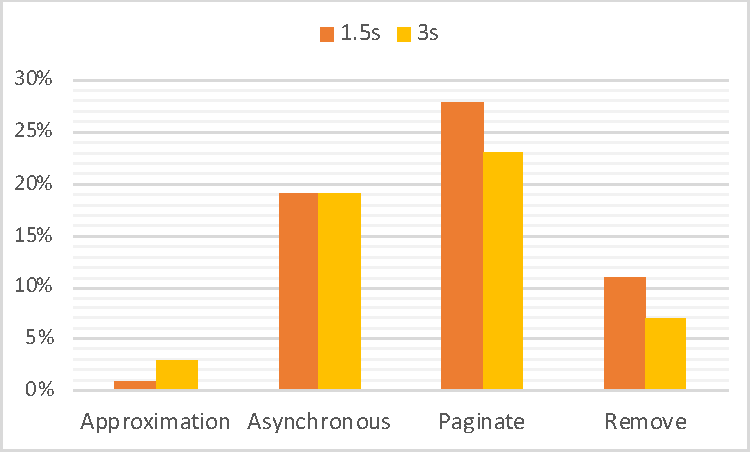
\includegraphics[width=0.8\columnwidth]{figs/preference.pdf}
    \caption{How much better do users like New pages?}
    \label{fig:userstudy_diff}
\end{figure}
\begin{figure}[h]
    \centering
    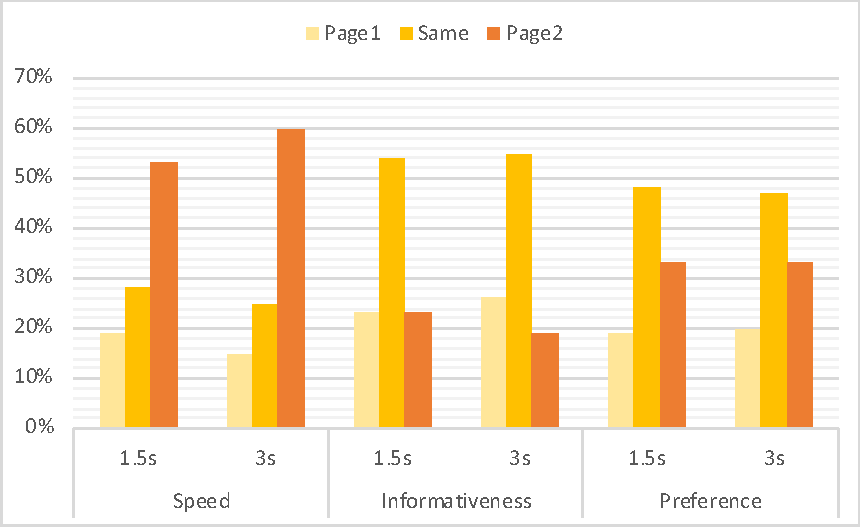
\includegraphics[width=0.8\columnwidth]{figs/user-study.pdf}
    \caption{How people prefer the pages?}
    \label{fig:userstudy}
\end{figure}
\fi

\subsubsection{User study results}
A summary of the user study results is shown in Table \ref{tab:userstudy_diff}, and the questionnaire and raw data are available on Panorama webpage \cite{userstudydata}.
%, there are always some participants who think Base is better, and some think New is better, and some think two versions are similar. \alvin{just say the results are mixed?}
In this table, we show the percentage of users who
think New is better minus those who think Base is better,
which we refer to as the {\it net} benefit of the new design, for every type of refactoring and every
question (Performance, Functionality, and Overall).
Users are given the two pages in random order, and are not aware of the view-design difference between the two pages in advance.

A short answer to our research question is ``Yes''. In fact, for all type
of view-changing optimization, users think the New design is {\it not worse}
than the Base design. Particularly, for {\it asynchronous} loading,
{\it pagination}, and {\it removal}, the new designs clearly win more users
than the baseline designs.

In terms of performance, the net win for the New design is clear. Many users
indeed notice the 1.5-second difference in the page-load time. In 10 out of 12 cases, \alvin{show \%?}
the New design has a net positive benefit on more than 30\% of the participants.

In terms of functionality, the results are quite interesting. For 
{\it approximation} and {\it pagination}, many users did notice the
content difference, leading to the Base design winning about 10\% of users.
However, for {\it asynchronous} loading and content {\it removal}, surprisingly,
many users neither notice the content difference nor think New design delivers worse contents. It could be that removing contents made the page cleaner to some users. For example, after removing the sidebar in Tracks \alvin{in Tracks? (if tracks is the app name)} (Tr5 in Table \ref{tab:dbsize} \alvin{I can't find case 11 in that table?}), some participants like it because ``Adding the sidebar makes scrolling harder.'' 

In terms of overall perception, the New design has a {\bf net win}.
Among the four types of optimizations, paginations and asynchronous loading
are the most appealing to users, while approximation is the least appealing.

We also conducted another set of user study with another 100 participants,
where we use an even larger (2-10$\times$) database size \alvin{how large?} \junwen{The size get differntly larger for different cases, some are 10 times, some are 2 times, some are 2.5 times} and hence make the page-load time
differences between New design and Base design even bigger (3 seconds).
We do observe that more participants noticed the performance advantage
of the New design. However, we also observe that the overall perception
only goes up a little bit more for the New design. We skip the details for
the space constraints.



\begin{table}[]

\centering
\caption{Net user perception enhancement by New design\\ (\% users 
who prefer New   $-$ \% users who prefer Base )}
\label{tab:userstudy_diff}
\begin{tabular}{@{}lrrrr@{}}
\toprule
                                & Approximation & Asynch & Paginate & Removal  \\ \midrule
Performance       & 23.50\%       & 31.00\%      & 45.00\%  & 35.50\% \\ 
%                             & 3s   & 35.50\%       & 42.00\%      & 45.50\%  & 58.00\% \\ \midrule
Functionality  & -7.50\%       & 17.50\%      & -13.00\% & 5.50\%  \\ 
 %                            & 3s   & -10.50\%       & 10.50\%      & -24.50\%  & -3.00\% \\ \midrule
Overall   & 1.00\%        & 18.50\%      & 28.00\%  & 10.50\% \\  
 %                            & 3s   & 2.50\%        & 19.00\%      & 23.00\%  & 7.00\%  \\ 
 \bottomrule
\end{tabular}
 \vspace{-0.2in}
\end{table}


\iffalse
\begin{table}[]
\centering				
\caption{User Study Result: Why prefers a web page?}
\label{tab:codebook}	\begin{tabular}{@{}clrm{3.5cm}@{}}
\toprule
                                            & Reason        & Num & Example                                           \\ \midrule
\multirow{3}{*}[-10pt]{Page 1}                     & Informative  & 125 & p1 has more  information.             \\ \cmidrule(l){2-4} 
                                            & Faster        & 37  & p1 loads fast.                                \\ \cmidrule(l){2-4} 
                                            & Display Style & 59  &  not paginating  is helpful. \\ \midrule
\multicolumn{1}{l}{\multirow{3}{*}[-10pt]{Page 2}} & Informative   & 83  & p2 has  more information.             \\ \cmidrule(l){2-4} 
\multicolumn{1}{l}{}                        & Faster        & 215 & p2 loads much faster.                         \\ \cmidrule(l){2-4} 
\multicolumn{1}{l}{}                        & Display Style & 168 & I like paginating.         \\ \bottomrule
\end{tabular}
\end{table}
\fi
\iffalse
\emph{Discussion.} The baseline page load time greatly affects people's attitude towards end-to-end time consumption. It's because of the non-uniform Internet status and human sense of time. In addition, longer loading time is, the more information on web-page the participant is expecting. During the experiment, we also found that participants have a strong preference towards pagination. Some of them think pagination is a clean UI design, while the others regard it as an obstacle to searching.
%[does the base line page-load time affect people's reaction?] [Does the users' reaction differ for different types of view-changes?]

\fi


\vspace{-0.05in}
\subsection{RQ4: how accurate is the \Tool estimator?}
We use the web page shown in Figure \ref{fig:heatmap} as a case study.
15 HTML tags on this page render dynamically generated contents.
With 200 database records, dynamic profiling shows that
the story tag is the top performance bottleneck, followed by the guideline
tag and then the message-count the cheapest. When the workload increases to
2000 and 20000 records, dynamic profiling shows that the guideline
tag is the top bottleneck, followed by the story tag. These results match
the performance gains we can get by optimizing these three tags: 
using 20000 records, asynchronously
loading or removing the guideline text can reduce the page end-to-end 
load time by more than 1 second; 
paginating the story-tag can speed up the page load time
by about 100 milliseconds; approximating the message count does not change page load time.

The static mode of \Tool estimator can indeed predict performance bottleneck
without running the application --- the guideline text gets the
highest complexity score (5) among all 15 tags, followed by the story tag (4), and then the
message-count tag (3), with the remaining 12 tags
getting 0 points.


\iffalse
\begin{table}[]
\centering
\caption{Performance cost ranking (static vs dynamic)}
\label{tab:cons1}
\begin{tabular}{@{}lrrrrrrr@{}}
\toprule
 & \multicolumn{2}{l}{200} & \multicolumn{2}{l}{2000} & \multicolumn{2}{l}{20000} & \multicolumn{1}{l}{static} \\ \midrule
guideline & \cellcolor[HTML]{C0C0C0}2 & 2 & \cellcolor[HTML]{C0C0C0}1 & 1 & \cellcolor[HTML]{C0C0C0}1 & 1 & 1 \\ \midrule
tags & \cellcolor[HTML]{C0C0C0}1 & 1 & \cellcolor[HTML]{C0C0C0}2 & 2 & \cellcolor[HTML]{C0C0C0}2 & 2 & 2 \\ \midrule
msg\_count & \cellcolor[HTML]{C0C0C0}3 & 3 & \cellcolor[HTML]{C0C0C0}3 & 3 & \cellcolor[HTML]{C0C0C0}3 & 3 & 3 \\ \bottomrule
\end{tabular}
\end{table}
\fi


%%%%%%COMMENT OUT%%%%
\begin{comment}

\begin{table}[]
\centering
{\small					
\caption{User Study Result: How people prefer the pages?}
\label{tab:userstudy}	
\begin{tabular}{@{}llrrrr@{}}
\toprule
 &  & \multicolumn{1}{l}{page1} & \multicolumn{1}{l}{same} & \multicolumn{1}{l}{page2} & \multicolumn{1}{l}{diff} \\ \midrule
Speed & 1.5s & 19.00\% & 28.25\% & 52.75\% & 33.75\% \\ \midrule
 & 3s & 15.13\% & 24.50\% & 60.38\% & 45.25\% \\ \midrule
Info&1.5s & 22.63\% & 54.13\% & 23.25\% & 0.63\% \\ \midrule
 & 3s & 26.00\% & 54.88\% & 19.13\% & -6.88\% \\ \midrule
Prefer & 1.5s & 18.88\% & 47.75\% & 33.38\% & 14.50\% \\ \midrule
 & 3s & 20.00\% & 47.13\% & 32.88\% & 12.88\% \\ \bottomrule
\end{tabular}
}
\end{table}

\end{comment}

\subsection{Threats to validity}
Threats to the validity of our work could come from multiple
sources. 
\textbf{Internal Validity}: The HTML tags that are dynamically generated through JavaScript can not be detected or analyzed by \Tool. \textbf{External Validity}: The 12 applications in our benchmark suite may not represent all real-world applications; The synthesized databases may not represent real-world workloads; The machine and network settings of our profiling may differ from real users’ setting; the 100 participants of our user-study from MTurk may not represent all real-world users. Overall, we have tried our best to conduct an unbiased study.


